\documentclass[hyperref={pdfpagelabels=true}]{beamer}
\usepackage{lmodern}
\usepackage{graphicx}
\usepackage{tikz}

%%%%%%%%%%%%%%%%%%%%%%%%%%%%%%%%%%%%%%%%%%%%%%%%%%%%%%%%%%%%%%%%%%%%%%%%%%%%%%%%%%%%%%%%%%%%%%%%%
%This work is licensed under a Creative Commons Attribution-ShareAlike 4.0 International License.
%
%You are free to:
%
%    Share — copy and redistribute the material in any medium or format
%    Adapt — remix, transform, and build upon the material
%    for any purpose, even commercially.
%
%    The licensor cannot revoke these freedoms as long as you follow the license terms.
%
%Attribution — You must give appropriate credit, provide a link to the license, and indicate if changes were made. You may do so in any reasonable manner, but not in any way that suggests the licensor endorses you or your use.
%
%ShareAlike — If you remix, transform, or build upon the material, you must distribute your contributions under the same license as the original. 
%
%%%%%%%%%%%%%%%%%%%%%%%%%%%%%%%%%%%%%%%%%%%%%%%%%%%%%%%%%%%%%%%%%%%%%%%%%%%%%%%%%%%%%%%%%%%%%%%%%
\definecolor{dred}{rgb}{0.647059, 0.164706, 0.164706}
\definecolor{dgreen}{rgb}{0., 0.545098, 0.545098}
%\usecolortheme[named=dred]{structure}

%\usetheme{Marburg}
%\usecolortheme{crane}

\usetheme{AnnArbor}
\usecolortheme{wolverine}

%\title{Horizontes no Panorama da Ci\^{e}ncia de Dados Espaciais}
\title{Ci\^{e}ncia de Dados Espaciais}
\subtitle{Aonde Vamos?}
\author{Joana Sim\~{o}es} 

\author[shortname]{Joana Sim\~{o}es \inst{1}}
\institute[shortinst]{\inst{1} Eurecat, Centro Tecnol\'{o}gico da Catalunha}

%\date{\today} 
\titlegraphic{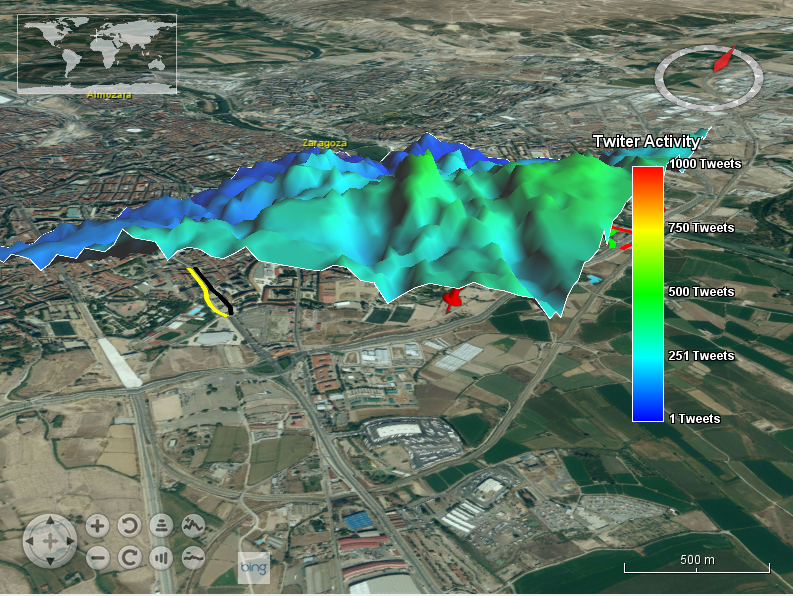
\includegraphics[width=.35\textwidth]{3d2.png}}

\usepackage{listings}

\newcommand{\soooo}{H$_2$SO$_4$}

%fdl stuff
\usepackage{hyperref}
\hypersetup{colorlinks, 
           citecolor=black,
           filecolor=black,
           linkcolor=black,
           urlcolor=black,
           bookmarksopen=true,
           pdftex}

\hfuzz = .6pt % avoid black boxes

\lstset{language=SQL}



\begin{document}
\setbeamertemplate{footline}[page number]
\setbeamertemplate{navigation symbols}{}

\titlepage

 
\begin{frame}
\frametitle{Tabela de Conte\'{u}dos}
\tiny{
\tableofcontents}
\end{frame}


\section{Introdu\c{c}\~{a}o} 
\begin{frame}
\frametitle{O que \'{e} a Ci\^{e}ncia de Dados?}

%TODO: explain what is data science

\end{frame}

\begin{frame}
\frametitle{Ci\^{e}ncia de Dados Espaciais}

%TODO: explain what is spatial data science

\end{frame}

\section{Tend\^{e}ncias} 
\begin{frame}
\frametitle{Onde Vamos?}

    \begin{figure}   
         
\includegraphics[width=0.7\textwidth]{fortune-teller.png}   
    \end{figure}     

\end{frame}


\begin{frame}
\frametitle{(Algumas) Tend\^{e}ncias}

    \begin{figure}   
         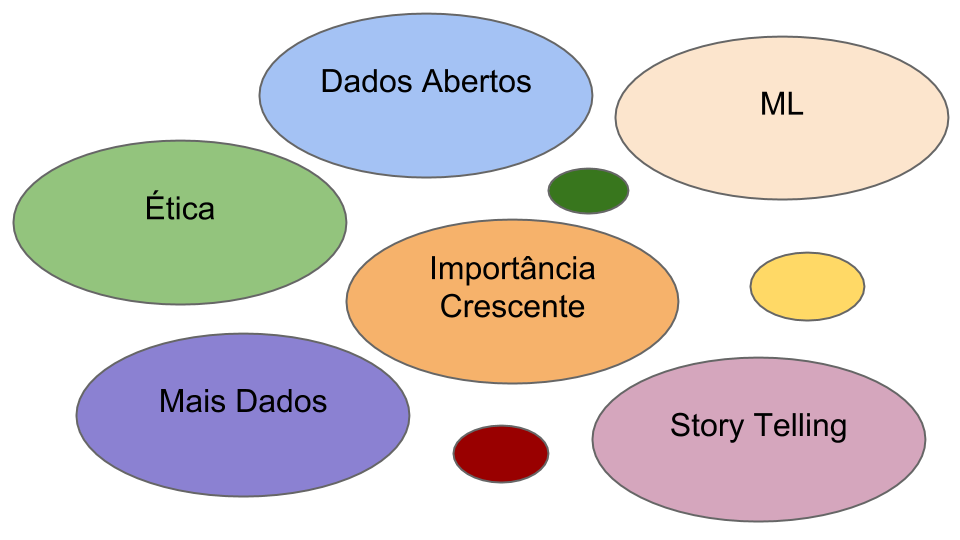
\includegraphics[width=\textwidth]{trends.png}   
    \end{figure}     

\end{frame}




\begin{frame}
\frametitle{Import\^{a}ncia Crescente}

%TODO: explain increasing scope

\end{frame}

\begin{frame}
\frametitle{Mais Dados}

%TODO: explain more data (automatic)

\end{frame}

\begin{frame}
\frametitle{E Ainda Mais Dados}

%TODO: explain more data (non-automatic)

\end{frame}

\begin{frame}
\frametitle{``Arqueologia'' de Dados}

%TODO: explain data archaeology

\end{frame}


\begin{frame}
\frametitle{Tecnologias de \textit{Big Data}}

%TODO: explain Big Data

\end{frame}

\begin{frame}
\frametitle{Uso Generalizado de \textit{Machine Learning}}

%TODO: explain ML

\end{frame}

\begin{frame}
\frametitle{Jornalismo de Dados \& \textit{Story Telling}}

%TODO: explain story telling
% visualizacao: em outro slide?

\end{frame}

\begin{frame}
\frametitle{Mais e Melhores Dados Abertos}

%TODO: explain Open Data

\end{frame}

\begin{frame}
\frametitle{\'{E}tica}

%TODO: spatial obfuscation

\end{frame}

\section{Consideracoes Finais} 
\begin{frame}
\frametitle{Resumo}

%TODO: resume the trends

\end{frame}

\begin{frame}
\frametitle{Import\^{a}ncia destas Tend\^{e}ncias para o FOSS4G}

%TODO: SIG Open-Source
%Free and Open Source Software for Geospatia

\end{frame}

\begin{frame}
\frametitle{Obrigada pela vossa Aten\c{c}\~{a}o}
    \begin{figure}   
      
\includegraphics[width=0.6\textwidth]{end.jpg}      
    \end{figure}   
    Esta apresenta\c{c}\~{a}o encontra-se dispon\'{i}vel em: \centering{\\ \url{http://tinyurl.com/nfbrhvl}\\}
      \vspace{5mm}    
\end{frame}


\end{document}


